
En la tabla~\tableref{table:table_sol_2} se muestra los primeros $5$ y los últimos $5$ valores de las soluciones del sistema del péndulo, la gráfica de las soluciones se puede ver en la figura~\figref{fig:fig_res_2}, para este segundo caso pedido, los parámetros del sistema son:

\begin{equation*}
                \begin{array}{ll}
                  m = 1 \si[per-mode=symbol]{\kilo\gram} \\
                  l = 1 \si[per-mode=symbol]{\meter} \\  
                  b = 0.5 \si[per-mode=symbol]{\newton\second\per\meter} \\ 
                  h = 0.2 \si[per-mode=symbol]{\second} \\   
                  \Theta_{0} = 30 \si[per-mode=symbol]{\degree} \\  
                  \dot{\Theta}_{0} = 100 \si[per-mode=symbol]{\degree\per\second} \\            
                \end{array}
\end{equation*}


\pgfkeys{
    /pgfplots/table/print last/.style={
        row predicate/.code={
            % Calculate where to start printing, use `truncatemacro` to get an integer without .0
            \pgfmathtruncatemacro\firstprintedrownumber{\pgfplotstablerows-#1} 
            \ifnum##1<\firstprintedrownumber\relax
                \pgfplotstableuserowfalse
            \fi
        }
    },
    /pgfplots/table/print last/.default=1
}


\pgfkeys{
    /pgfplots/table/print middle/.style={
        row predicate/.code={
            % Calculate where to start printing, use `truncatemacro` to get an integer without .0
            \pgfmathtruncatemacro\firstprintedrownumber{\pgfplotstablerows-#1} 
            \pgfmathtruncatemacro\lastprintedrownumber{#1-1} 
            \ifnum##1>\lastprintedrownumber\relax
                \ifnum##1<\firstprintedrownumber\relax
                    \pgfplotstableuserowfalse
                \fi
            \fi
        }
    },
    /pgfplots/table/print last/.default=1
}



\begin{center}

\pgfplotstableset{
begin table=\begin{longtable},
end table=\end{longtable},
}

\pgfplotstabletypeset[
    print middle=5,
    col sep=comma,
    multicolumn names, 
%%	
    every head row/.style={before row={\toprule \rowcolor{LightOrange}}, 
    after row={\toprule\toprule}},
%%		
    every last row/.style={after row={\bottomrule \caption{\label{table:table_sol_2}
    \footnotesize{Tabla de salida para el algoritmo de Runge-Kutta 4 para el primer caso.}}}},		
%%		
    every row/.style={after row=\hline},
%%		
    every even row/.style={before row={\rowcolor{Lightblue2}}},  
%%	
    every row no 5/.style={before row={\toprule\toprule}},    
%%		
    columns/0/.style={
		column name={Tiempo $\left[ \si[per-mode=symbol]{\second} \right]$},
		string type,
		column type={S[round-precision=10, round-mode=places, scientific-notation=false, group-digits=false, table-align-text-pre=true, detect-mode,
        tight-spacing=true]}},
%%		
    columns/1/.style={
		column name={$\Theta \left[ \si[per-mode=symbol]{\radian} \right]$},
		string type,
		column type={S[round-precision=15, round-mode=places, scientific-notation=false, group-digits=false, table-align-text-pre=true, detect-mode,
        tight-spacing=true]}},
%%		
    columns/2/.style={
		column name={$\dot{\Theta} \left[ \si[per-mode=symbol]{\radian\per\second} \right]$},
		string type,
		column type={S[round-precision=15, round-mode=places, scientific-notation=false, group-digits=false, table-align-text-pre=true, detect-mode,
        tight-spacing=true]}},
%%	
%    skip rows between index={5}{\pgfplotstablerows-5}
%%	
    ]{results/valores_respuesta_2.csv}
    
\end{center}  


Para este caso el valor obtenido para la integral del módulo de la posición por el método de Romberg es: 


\[
 \highlight{LightOrange}{I = 2.7320644496497102}
\]

Vale lo mismo dicho anteriormente para el error.


\clearpage


\begin{figure}[H] %htb
\begin{center}
\makebox[\textwidth]{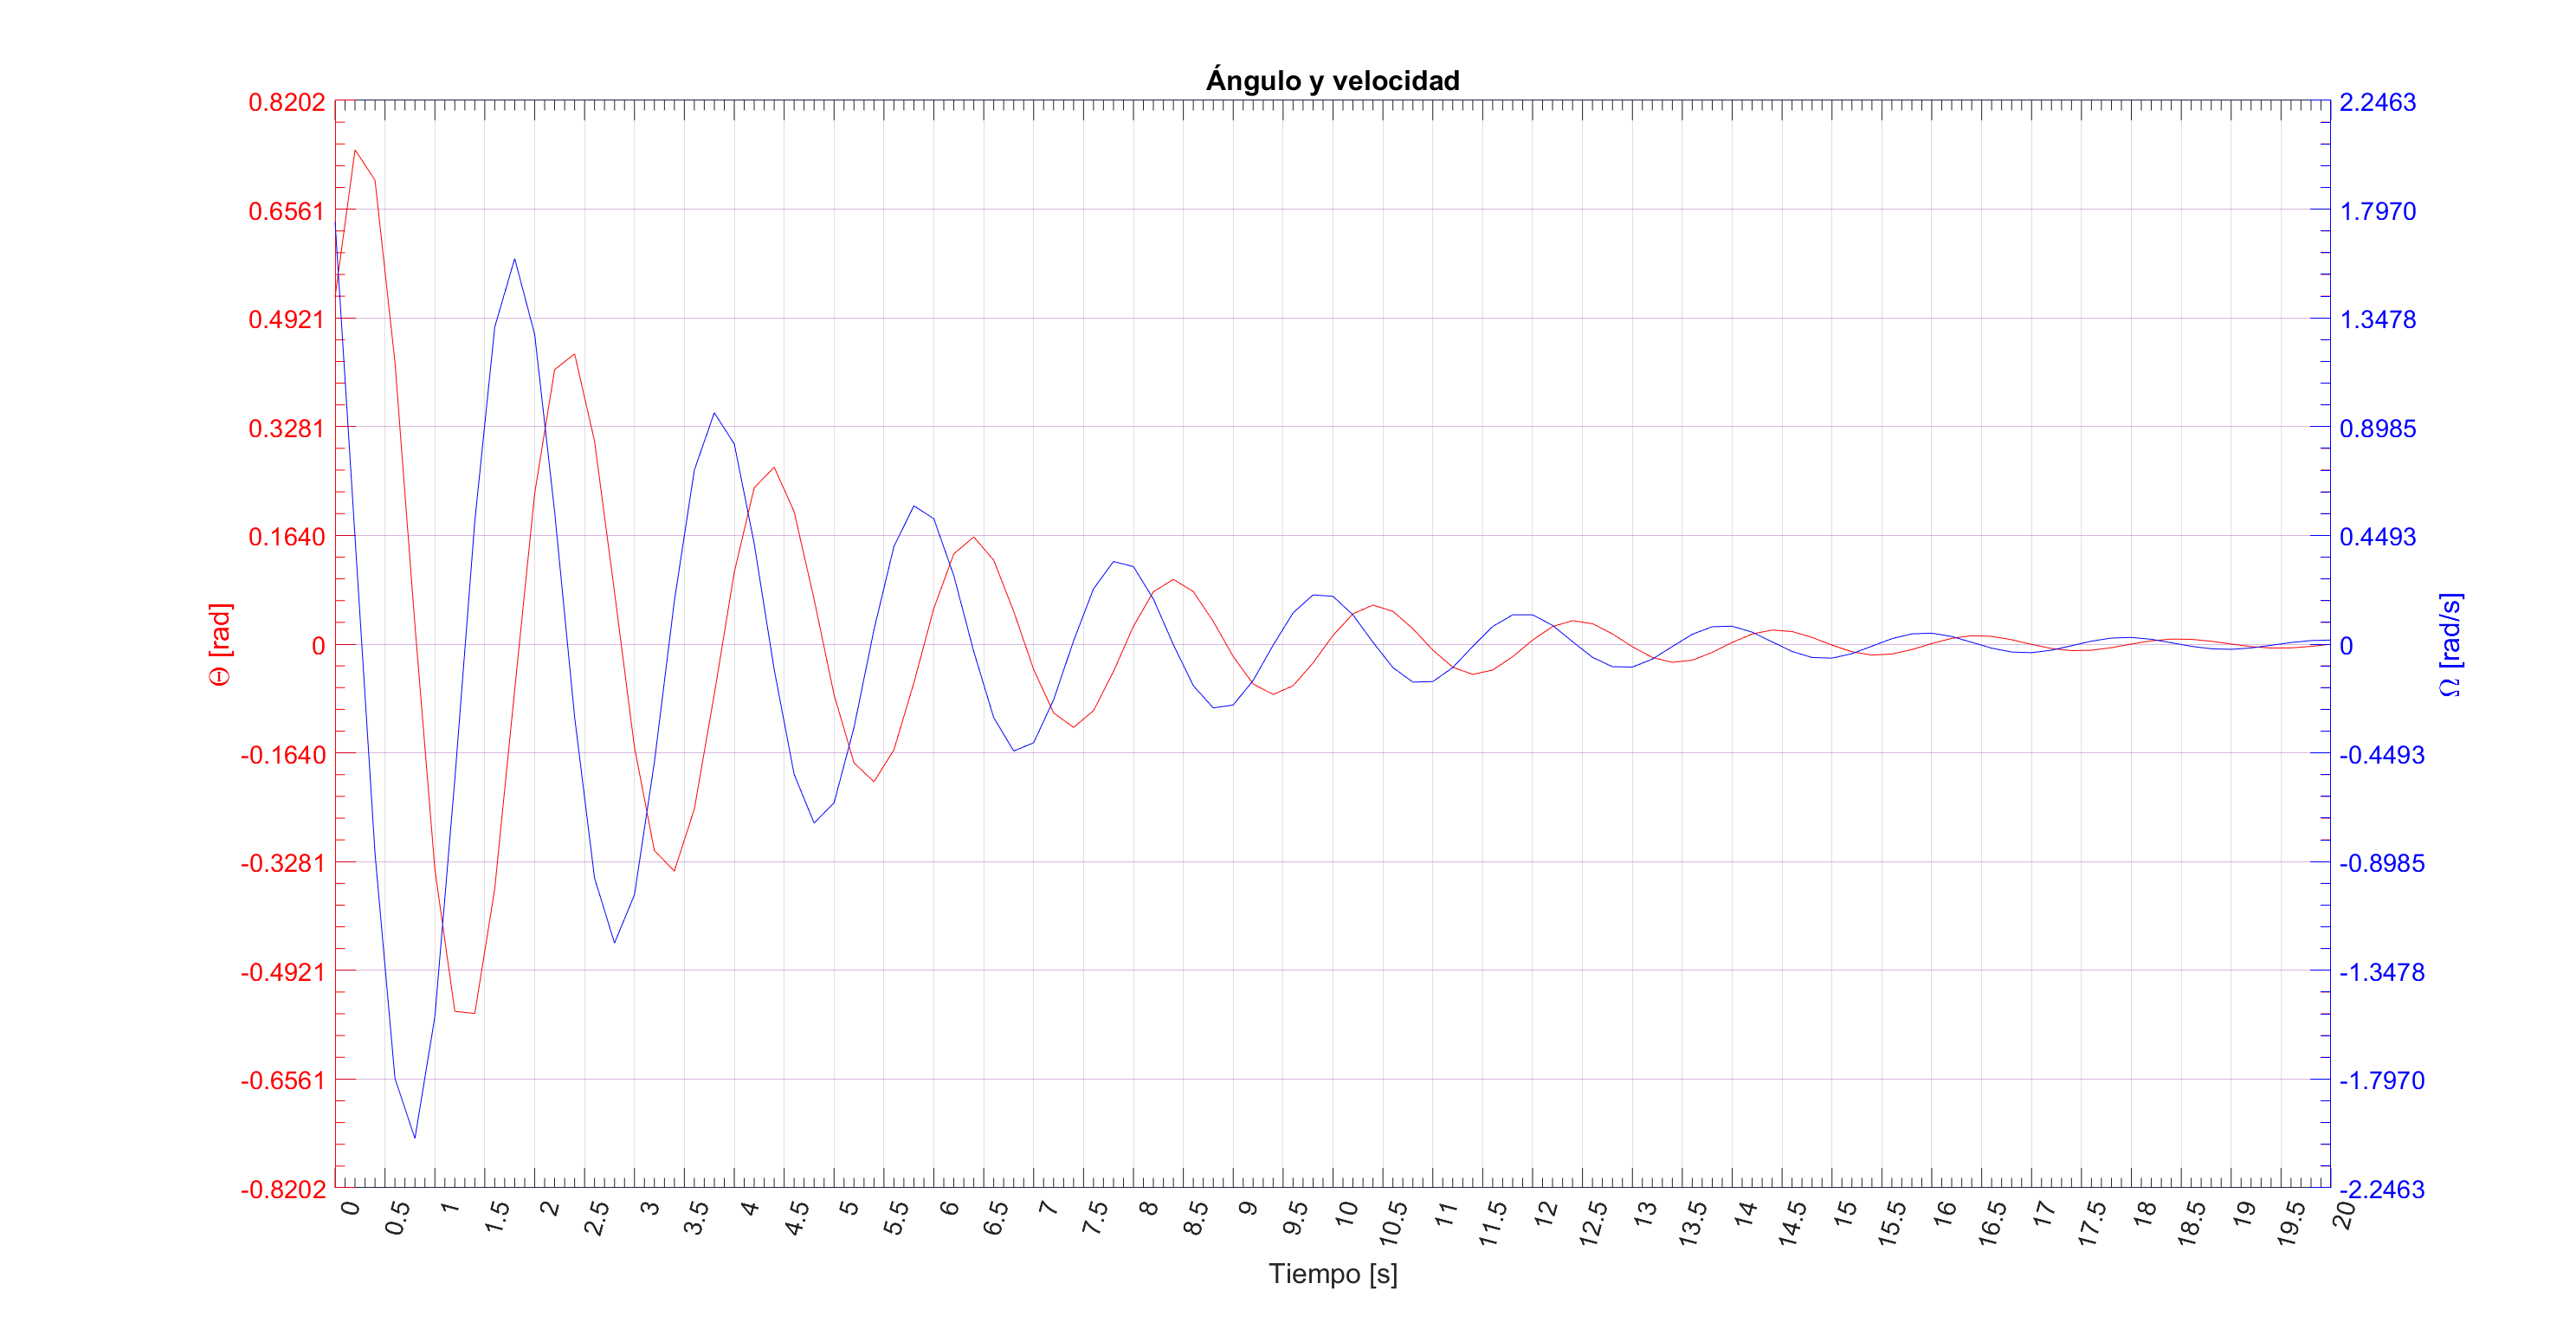
\includegraphics[width=0.95 \paperwidth,keepaspectratio=true, angle=90]{img/grafico_respuesta_2.png}} %% 
\caption{\label{fig:fig_res_2}\footnotesize{Gráfico de la solución para el primer caso.}}
\end{center}
\end{figure}



